\chapter{the \texorpdfstring{$m_1 + m_2$}{m1 + m2} decomposition of spacetime}
\begin{itemize}
	\item 将 $n$-dim. 流形分解为 $m_1 + m_2$ 维 ($m_1 + m_2 = n$), 其中 $m_2$ 是超曲面的维数.
	
	\item 选取与超曲面 "适配" 的坐标, $\{\chi^1, \cdots, \chi^{m_1}, \xi^1, \cdots, \xi^{m_2}\}$, 即超曲面上的点的前 $m_1$ 个坐标值为常数.
	\begin{itemize}
		\item 用 $\alpha, \beta, \gamma = 1, \cdots, m_1$, 以及 $i, j, k = m_1 + 1, \cdots, n$.
	\end{itemize}
	
	\begin{figure}[H]
		\centering
		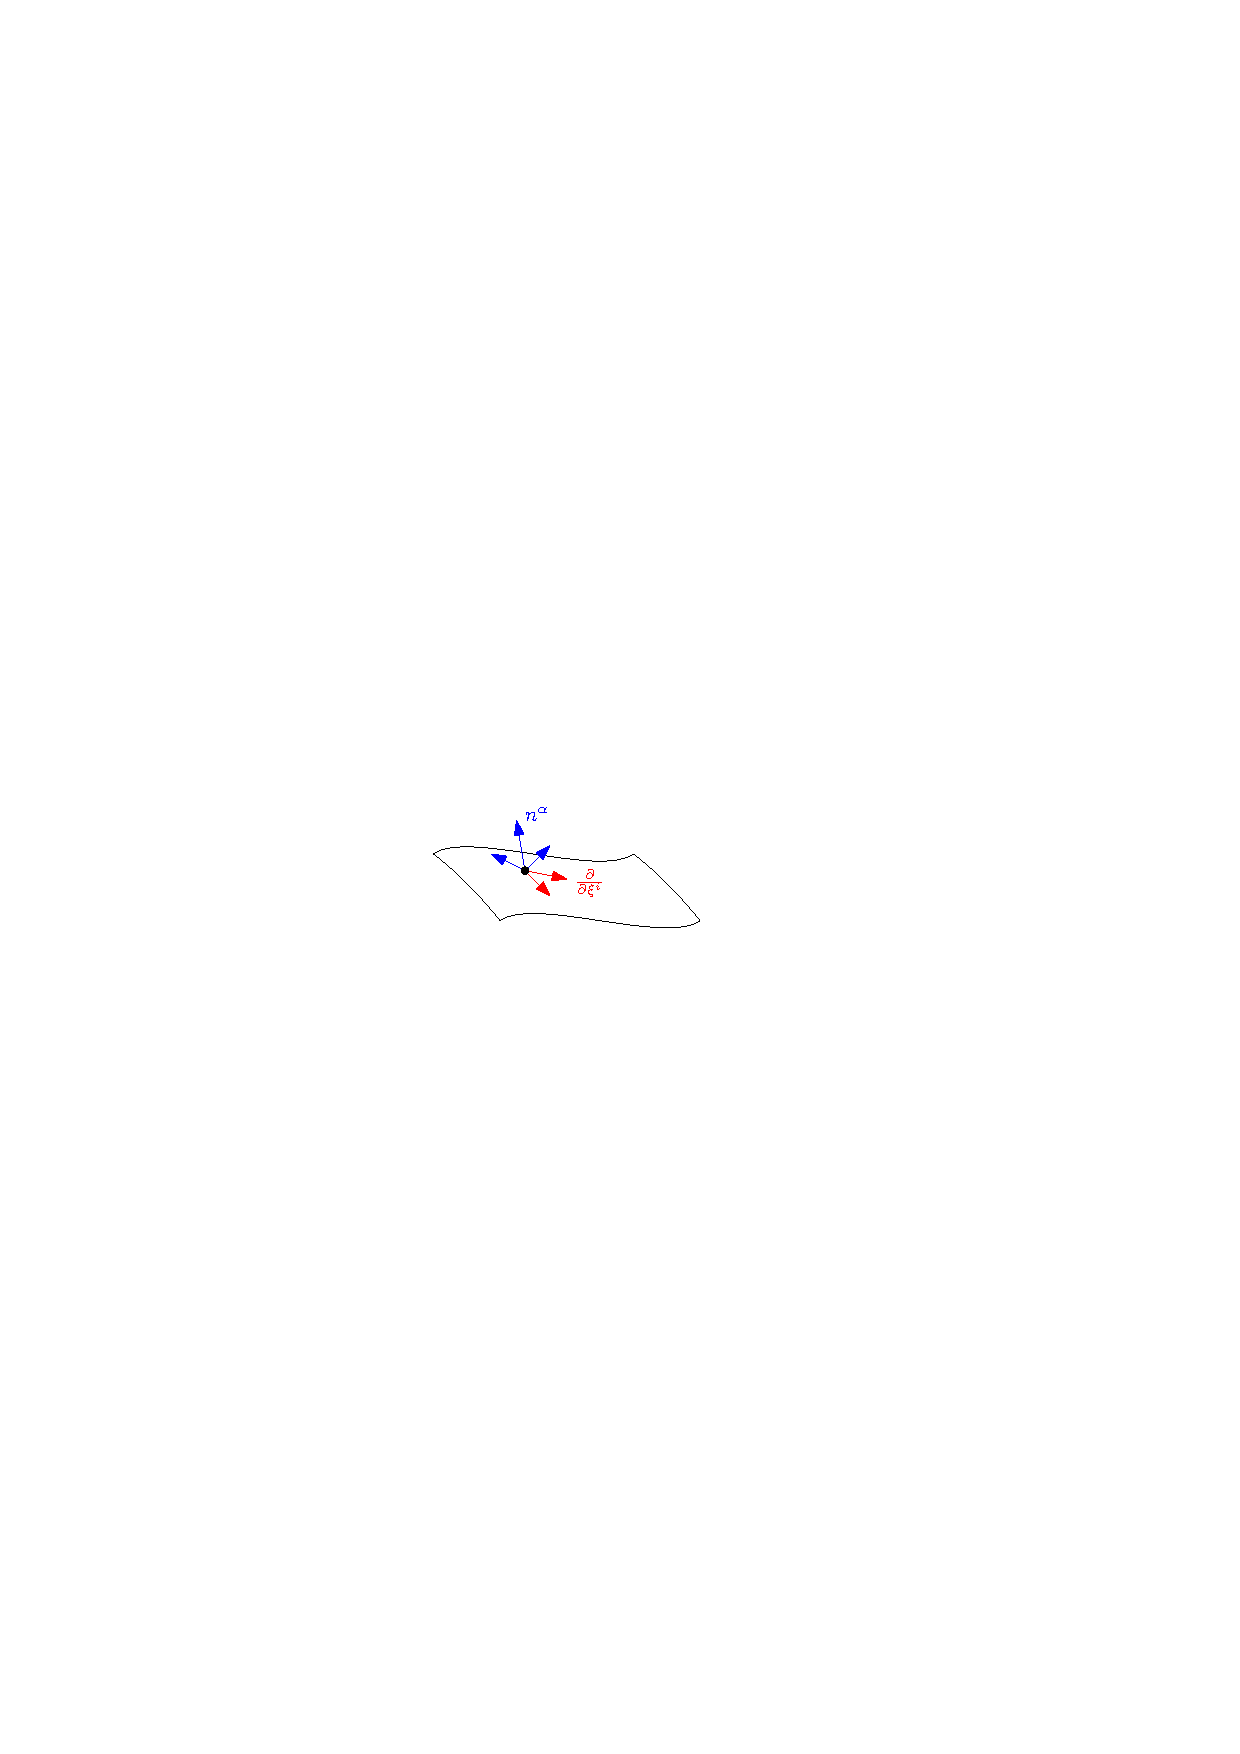
\includegraphics[scale=1]{figures/the m1 + m2 decomposition of spacetime.pdf}
	\end{figure}
\end{itemize}

\section{induced metric}
\begin{itemize}
	\item 对 $d\chi^1, \cdots, d\chi^{m_1}$ 进行 Schmidt 正交化并归一化, 得到 $n^1, \cdots, n^{m_1}$, 有,
	\begin{equation}
		(n^\alpha)^a (n^\alpha)_a = \epsilon^\alpha = \pm 1
	\end{equation}
	
	\item 投影张量为,
	\begin{equation}
		{h^a}_b = \delta^a_b - \sum_\alpha \epsilon^\alpha (n^\alpha)^a (n^\alpha)_b
	\end{equation}
	
	\item 因此, 诱导度规为,
	\begin{equation} \label{C.1.3}
		h_{a b} = {h^c}_a {h^d}_b g_{c d} = g_{a b} - \sum_\alpha \epsilon^\alpha (n^\alpha)_a (n^\alpha)_b
	\end{equation}
	\begin{itemize}
		\item 另外,
		\begin{equation}
			h^{a b} = g^{a b} - \sum_\alpha \epsilon^\alpha (n^\alpha)^a (n^\alpha)^b
		\end{equation}
		
		\item 且有 $h^{a c} h_{b c} = {h^a}_b$.
	\end{itemize}
\end{itemize}

\section{the decomposition}
\begin{itemize}
	\item \textbf{def.:} 定义系数 $N^{\alpha \beta}, M^{\alpha i}$ 如下,
	\begin{equation}
		\Big( \frac{\partial}{\partial \chi^\alpha} \Big)^a = \sum_\beta N^{\alpha \beta} (n^\beta)^a + \sum_i M^{\alpha i} \Big( \frac{\partial}{\partial \xi^i} \Big)^a
	\end{equation}
	\begin{itemize}
		\item 有,
		\begin{equation} \label{C.2.2}
			N^{\alpha \beta} = \epsilon^\beta (n^\beta)_a \Big( \frac{\partial}{\partial \chi^\alpha} \Big)^a
		\end{equation}
	\end{itemize}
	
	\item 那么,
	\begin{align}
		& g_{\mu \nu} = \begin{pmatrix}
			\epsilon^\gamma N^{\alpha \gamma} N^{\beta \gamma} + M^{\alpha i} M^{\beta j} g_{i j} & \{M^{\alpha j} g_{j i}\}^T \\
			M^{\alpha j} g_{j i} & g_{i j}
		\end{pmatrix} \\
		\Longrightarrow & \det \{g_{\mu \nu}\} = \det \{\epsilon^\gamma N^{\alpha \gamma} N^{\beta \gamma}\} \det \{g_{i j}\}
	\end{align}
	
	\begin{tcolorbox}[title=calculation:]
		注意到 $(n^\alpha)_a \big( \frac{\partial}{\partial \xi^i} \big)^a = 0$, 且 $g_{a b} (n^\alpha)^a (n^\beta)^b = \epsilon^\alpha \delta_{\alpha \beta}$, 所以...
	\end{tcolorbox}
\end{itemize}

\section{induced volume form}
\begin{itemize}
	\item \textbf{def.:} 令,
	\begin{equation}
		g = |\det \{g_{\mu \nu}\}| \quad \epsilon N^2 = \det \{\epsilon^\gamma N^{\alpha \gamma} N^{\beta \gamma}\} \quad h = |\det \{h_{i j}\}|
	\end{equation}
	其中, 根据 \eqref{C.1.3}, 有 $h_{i j} = g_{i j}$.
	
	\item 那么,
	\begin{equation}
		g = N^2 h \iff \sqrt{h} = \frac{\sqrt{g}}{N}
	\end{equation}
	
	\item the induced volume form is,
	\begin{align}
		\tilde{\epsilon} &= \sqrt{h} \underbrace{{h_{a_1}}^{b_1} (d\xi^1)_{b_1}}_{= (d\xi^1)_{a_1} - \sum_\alpha \epsilon^\alpha (n^\alpha)_{a_1} (n^\alpha)^{b_1} (d\xi^1)_{b_1}} \wedge \cdots \wedge {h_{a_{m_2}}}^{b_{m_2}} (d\xi^{m_2})_{b_{m_2}} \notag \\
		&= \frac{\sqrt{g}}{N} \Big( (d\xi^1)_{b_1} \wedge \cdots \wedge (d\xi^{m_2})_{b_{m_2}} - \big( \epsilon^\alpha (n^\alpha)^{b_1} (d\xi^1)_{b_1} \big) (n^\alpha)_{a_1} \wedge \cdots \wedge (d\xi^{m_2})_{b_{m_2}} - \cdots \Big) \label{C.3.3}
	\end{align}
	注意到,
	\begin{equation} \label{C.3.4}
		\epsilon = \sqrt{g} \underbrace{d\chi^1 \wedge \cdots d\chi^{m_1}}_{= \frac{1}{N} n^1 \wedge \cdots \wedge n^{m_1}} \wedge d\xi^1 \wedge \cdots \wedge d\xi^{m_2}
	\end{equation}
	对比 \eqref{C.3.3} 和 \eqref{C.3.4}, 所以,
	\begin{equation}
		\epsilon = n^1 \wedge \cdots \wedge n^{m_1} \wedge \tilde{\epsilon} \Longrightarrow \tilde{\epsilon} = \frac{\prod_\alpha \epsilon^\alpha}{m_1 !} (n^1)^{b_1} \wedge \cdots \wedge (n^{m_1})^{b_{m_1}} \epsilon_{b_1 \cdots b_{m_1} a_1 \cdots a_{m_2}}
	\end{equation}
	\begin{itemize}
		\item 其中, 我们还需要证明 $d\chi^1 \wedge \cdots d\chi^{m_1} = \frac{1}{N} n^1 \wedge \cdots \wedge n^{m_1}$.
		
		\begin{tcolorbox}[title=proof:]
			根据 \eqref{C.2.2}, 可知 Schmidt 正交化并归一化的系数为,
			\begin{equation}
				n^\alpha = \sum_\beta N^{\alpha \beta} d\chi^\beta
			\end{equation}
			
			\noindent\rule[0.5ex]{\linewidth}{0.5pt} % horizontal line
			
			$N^{\alpha \beta}$ 的两条性质 (并不重要),
			\begin{itemize}
				\item 考虑到归一化条件, 有,
				\begin{equation}
					\sum_{\gamma, \delta} g^{\gamma \delta} N^{\alpha \gamma} N^{\beta \delta} = \epsilon^\alpha \delta_{\alpha \beta} \iff N \cdot \{g^{\alpha \beta}\} \cdot N^T = \begin{pmatrix}
						\epsilon^1 & & \\
						& \ddots & \\
						& & \epsilon^{m_1}
					\end{pmatrix}
				\end{equation}
				
				\item 另外, 注意到 \eqref{C.2.2}, 有,
				\begin{align}
					& N^{\alpha \beta} = \epsilon^\beta \sum_\gamma N^{\beta \gamma} (d\chi^\gamma)_a \Big( \frac{\partial}{\partial \chi^\alpha} \Big)^a \notag \\
					\Longrightarrow & N^T = \mathrm{diag}(\epsilon^1, \cdots, \epsilon^{m_1}) \cdot N
				\end{align}
			\end{itemize}
			
			\noindent\rule[0.5ex]{\linewidth}{0.5pt} % horizontal line
			
			所以,
			\begin{align}
				n^1 \wedge \cdots \wedge n^{m_1} &= N^{1 \alpha_1} d\chi^{\alpha_1} \wedge \cdots \wedge N^{m_1 \alpha_{m_1}} d\chi^{\alpha_{m_1}} \notag \\
				&= \underbrace{\det N}_{= N} \, d\chi^1 \wedge \cdots \wedge d\chi^{m_1}
			\end{align}
		\end{tcolorbox}
	\end{itemize}
\end{itemize}
